%\documentclass{article}
%\usepackage{graphicx}
%\usepackage{url}
%\graphicspath{/home/Chinmayee/MM/Assignment-4/tex document/}
%\title{Newton's Second Law}
%\author{Chinmayee}

%\begin{document}
\section{Chinmayee - ME20B053}
\subsection{Newton's Second Law} \cite{Newton_second_law}

\begin{equation}
F=ma (= change in momentum)
\end{equation}

%\begin{description}
$F$ = Force acting on the body \\
$m$ = Mass of the body \\
$a$ = Acceleration of the body \\
%\end{description}

\paragraph{}
Newton's second law states that the acceleration of an object is directly related to the net force and inversely related to its mass. Acceleration of an object depends on two things, force and mass. It allows you to calculate the acceleration (and therefore velocity and position) of an object with known forces. The force acting on a body is equal to the change in momentum of the body per unit time, which in turn gives us "F=ma".  

\begin{figure}[!ht]
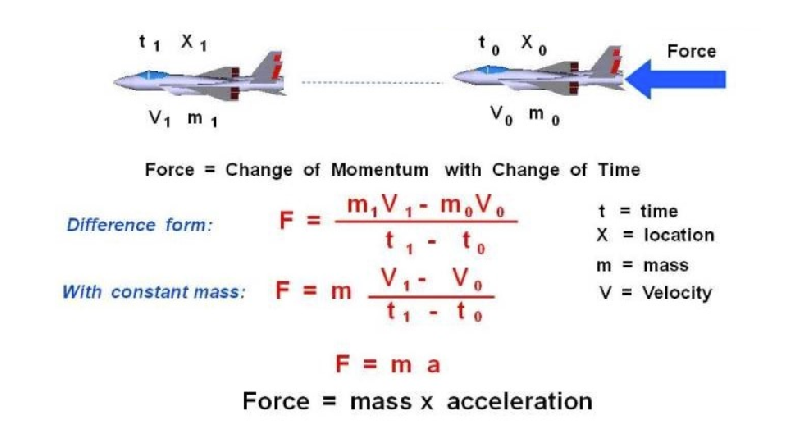
\includegraphics[width=350px]{me20b053/me20b053.eps}
\caption{ME20B053} \cite{Newton_discription}
\label{fig : Newton's Second Law}
\end{figure}

%\bibliography{team-3.bib}
%\bibliographystyle{plain}

%\end{document}
